\documentclass{article}
\usepackage{geometry}
\geometry{margin=1.5cm, vmargin={0pt,1cm}}
\setlength{\topmargin}{-1cm}
\setlength{\paperheight}{29.7cm}
\setlength{\textheight}{25.3cm}

% useful packages.
\usepackage{amsfonts}
\usepackage{amsmath}
\usepackage{amssymb}
\usepackage{amsthm}
\usepackage{enumerate}
\usepackage{graphicx}
\usepackage{multicol}
\usepackage{fancyhdr}
\usepackage{layout}
% \usepackage{ctex}
\usepackage{listings}
\usepackage{subfigure}
\usepackage{setspace}

% some common command
\newcommand{\dif}{\mathrm{d}}
\newcommand{\avg}[1]{\left\langle #1 \right\rangle}
\newcommand{\difFrac}[2]{\frac{\dif #1}{\dif #2}}
\newcommand{\pdfFrac}[2]{\frac{\partial #1}{\partial #2}}
\newcommand{\OFL}{\mathrm{OFL}}
\newcommand{\UFL}{\mathrm{UFL}}
\newcommand{\fl}{\mathrm{fl}}
\newcommand{\op}{\odot}
\newcommand{\Eabs}{E_{\mathrm{abs}}}
\newcommand{\Erel}{E_{\mathrm{rel}}}
\newcommand{\RNum}[1]{\uppercase\expandafter{\romannumeral #1\relax}}

\usepackage{xcolor}
\usepackage{fontspec} 
\definecolor{dkgreen}{rgb}{0,0.6,0}
\definecolor{gray}{rgb}{0.5,0.5,0.5}
\definecolor{comment}{rgb}{0.56,0.64,0.68}

\newfontfamily\monaco{Monaco}
\lstset {
aboveskip=3mm,
belowskip=3mm,
showstringspaces=false,       % underline spaces within strings
columns=flexible,
framerule=1pt,
rulecolor=\color{gray!35},
backgroundcolor=\color{gray!5},
basicstyle={\small\monaco},           % the size of the fonts that are used for the code
numbers=left,                   % where to put the line-numbers
numberstyle=\tiny\monaco\color{gray},  % the style that is used for the line-numbers
numbersep=5pt,                  % how far the line-numbers are from the code
commentstyle=\color{comment},
keywordstyle=\color{blue},
stringstyle=\color{dkgreen},
tabsize=2,                      % sets default tabsize to 2 spaces
captionpos=b,                   % sets the caption-position to bottom
breaklines=true,                % sets automatic line breaking
breakatwhitespace=false,        % sets if automatic breaks should only happen at whitespace
escapeinside={\%*}{*)},            % if add LaTeX within your code
morekeywords={*,...}               % if add more keywords to the set
}


\begin{document}
\title{Homework \#3}
\pagestyle{fancy}
\lhead{Name Li HuiTeng 3180102114}
\chead{ NumAnalysis\#3}
\rhead{Date 21.11.17}

\section{Theoretical questions}
This part can be found in Latex Folder.

\section{C++ programming}
Follow the $\textbf{readme}$, and generate all answers! 
Codes are contained in the e-mail tar, and only conclusions will be shown in the following part.

\subsection{\textbf{Structure of codes}}
$\textbf{bin}$ stores compiled files;\\
$\textbf{doc}$ stores the same document as this one;\\
$\textbf{include}$ stores sources files that support spline implementation;\\
$\textbf{main}$ stores files concerning the assignments;\\
$\textbf{output}$ stores all results such as $\textbf{*.m}$ and $\textbf{*.png}$.\\
$\textbf{test}$ stores test files.\\
Results for each part are shown below, generating from $ \textbf{make runAssignment} $ and $ \textbf{make plotAssignment} $.
\subsection{\textbf{Assignment B}}
\lstset{language=C++}
\begin{lstlisting}
  ------------------------Assignment B--------------------------
  For Complete situation, 
  N = 6, error_max = 0.421705, convergence rate = 5.35038
  N = 11, error_max = 0.0103367, convergence rate = 2.16165
  N = 21, error_max = 0.00231026, convergence rate = 3.06868
  N = 41, error_max = 0.000275356, convergence rate = 4.09706
  N = 81, error_max = 1.609e-05
  For Not_a_knot situation, 
  N = 6, error_max = 0.431538, convergence rate = 5.38047
  N = 11, error_max = 0.0103594, convergence rate = 2.16482
  N = 21, error_max = 0.00231026, convergence rate = 3.06869
  N = 41, error_max = 0.000275356, convergence rate = 4.09706
  N = 81, error_max = 1.609e-05
  Plots have been generated as '/output/B_[XX]Plot.m'.
\end{lstlisting}
After plotting, we have

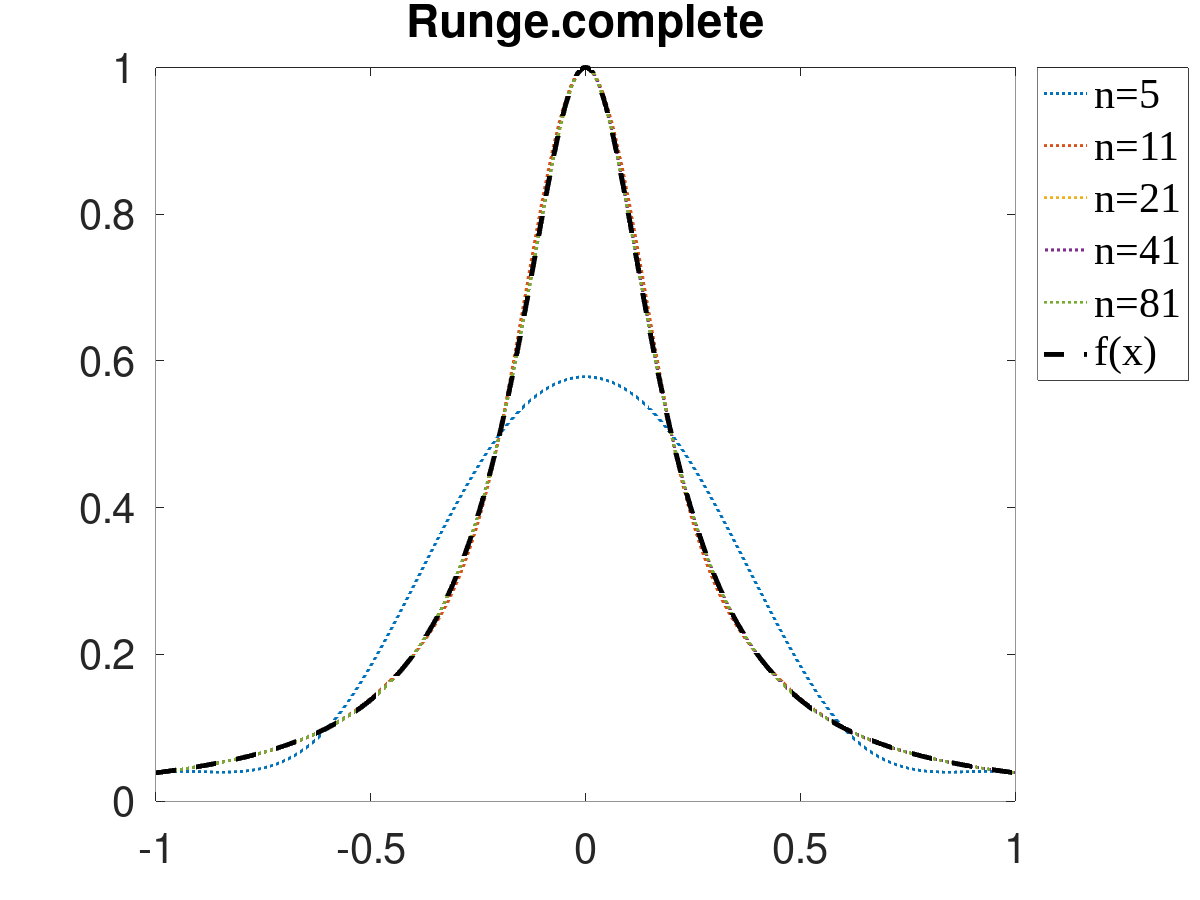
\includegraphics[width=0.45\textwidth]{../output/Assignment_B_complete.png}
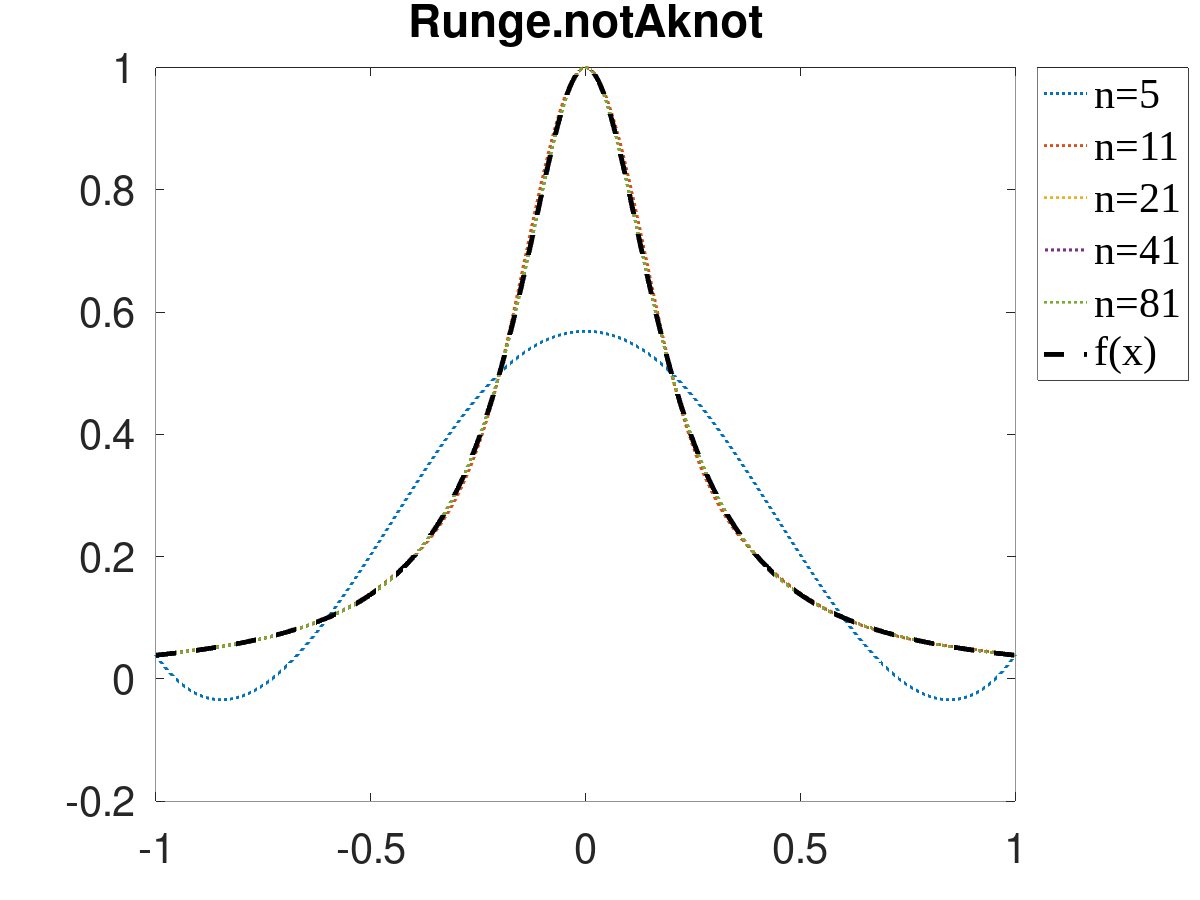
\includegraphics[width=0.45\textwidth]{../output/Assignment_B_notAknot.png}

The results show spline interpolation is indeed free of the wide oscillations in the Runge phenomenon.

\subsection*{\textbf{Assignment C and D}}
\lstset{language=C++}
\begin{lstlisting}
  ------------------------Assignment C--------------------------
  Plots have been generated as '/output/C_[XX].m'.
  ------------------------Assignment D--------------------------
  x = -3.5: E_458 = 0.000669568, E_459 = 0
  x = -3: E_458 = 0, E_459 = 0.00141838
  x = -0.5: E_458 = 0.0205289, E_459 = 1.11022e-16
  x = 0: E_458 = 1.11022e-16, E_459 = 0.120238
  x = 0.5: E_458 = 0.0205289, E_459 = 1.11022e-16
  x = 3: E_458 = 0, E_459 = 0.00141838
  x = 3.5: E_458 = 0.000669568, E_459 = 0
\end{lstlisting}
After plotting, we have

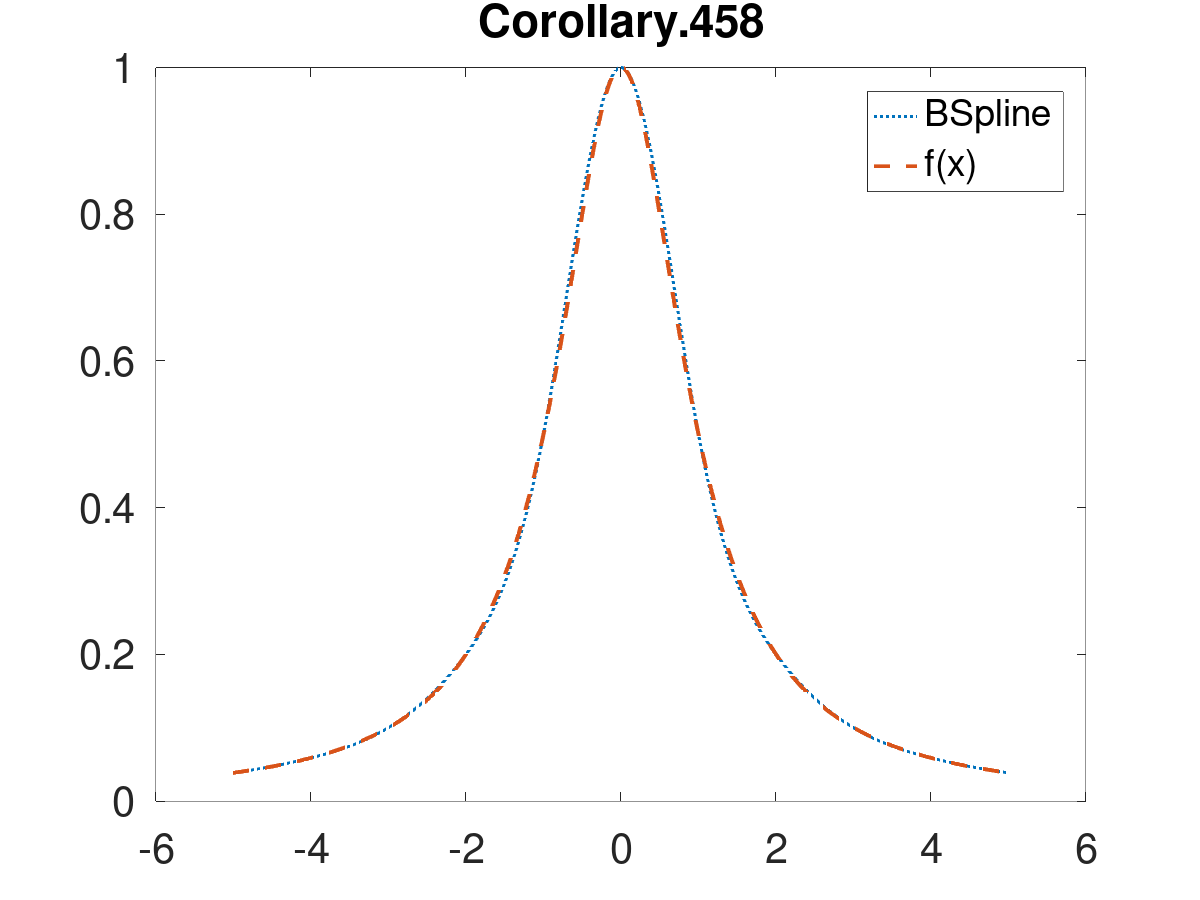
\includegraphics[width=0.45\textwidth]{../output/Assignment_C_458.png}
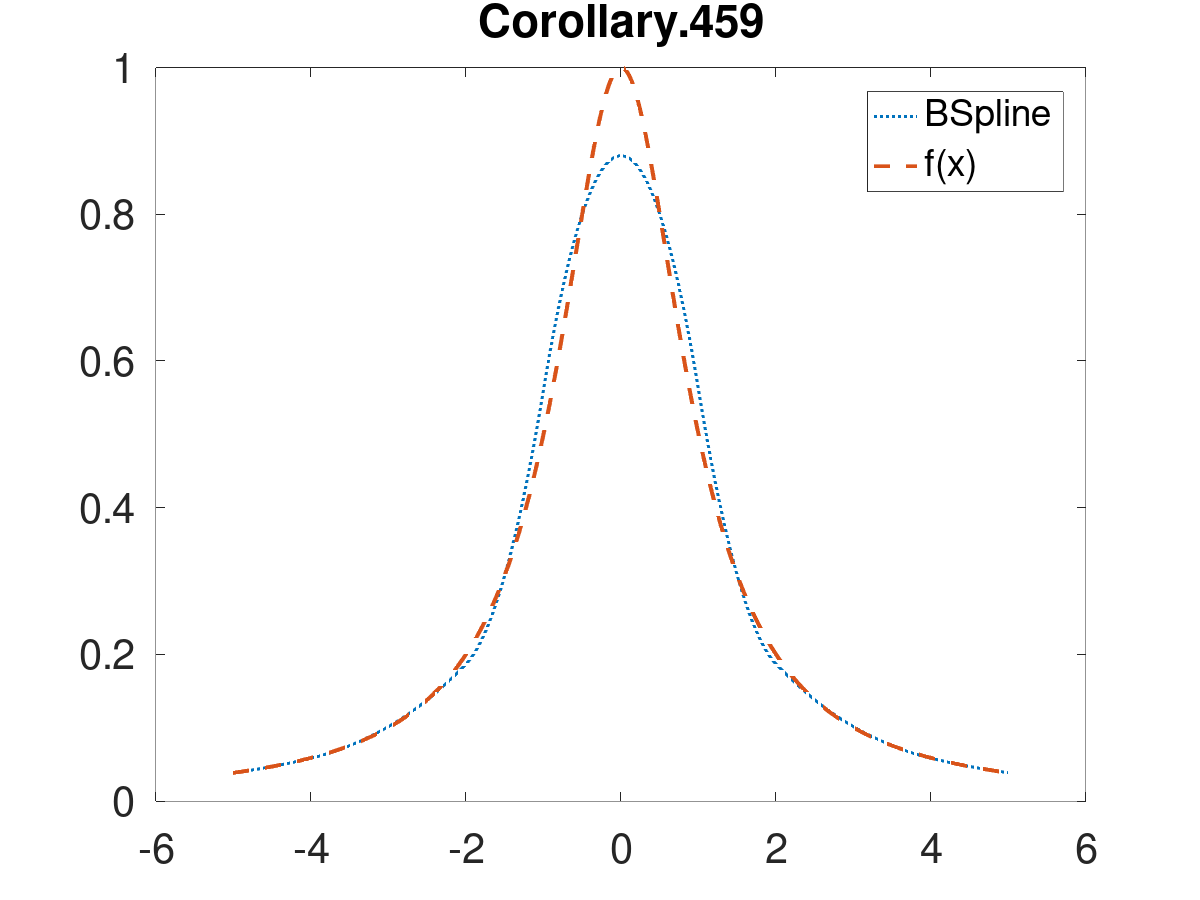
\includegraphics[width=0.45\textwidth]{../output/Assignment_C_459.png}

which answer \textbf{Assignment C}.

For \textbf{Assignment D}, it's trivial to see that the interpolation spline will have 
its error close to machine precision on its interpolation sites, since the function values 
on those points are given as preconditions and used as the RHS of linear equations that any 
solution shall satisfy. 

Also, from the maximums of middle point errors and the above plots, the first B-spline, a complete cubic 
cardinal B-spline, is more accurate.

\subsection{\textbf{Assignment E}}
\lstset{language=C++}
We apply \textbf{Spline<2,4,ppForm> fitCurve} with \textbf{BCType = periodic} since it's 
a simple close curve. 
\begin{lstlisting}
  ------------------------Assignment E--------------------------
  Plots have been generated as '/output/E_[XX].m'.
\end{lstlisting}
After plotting, we have

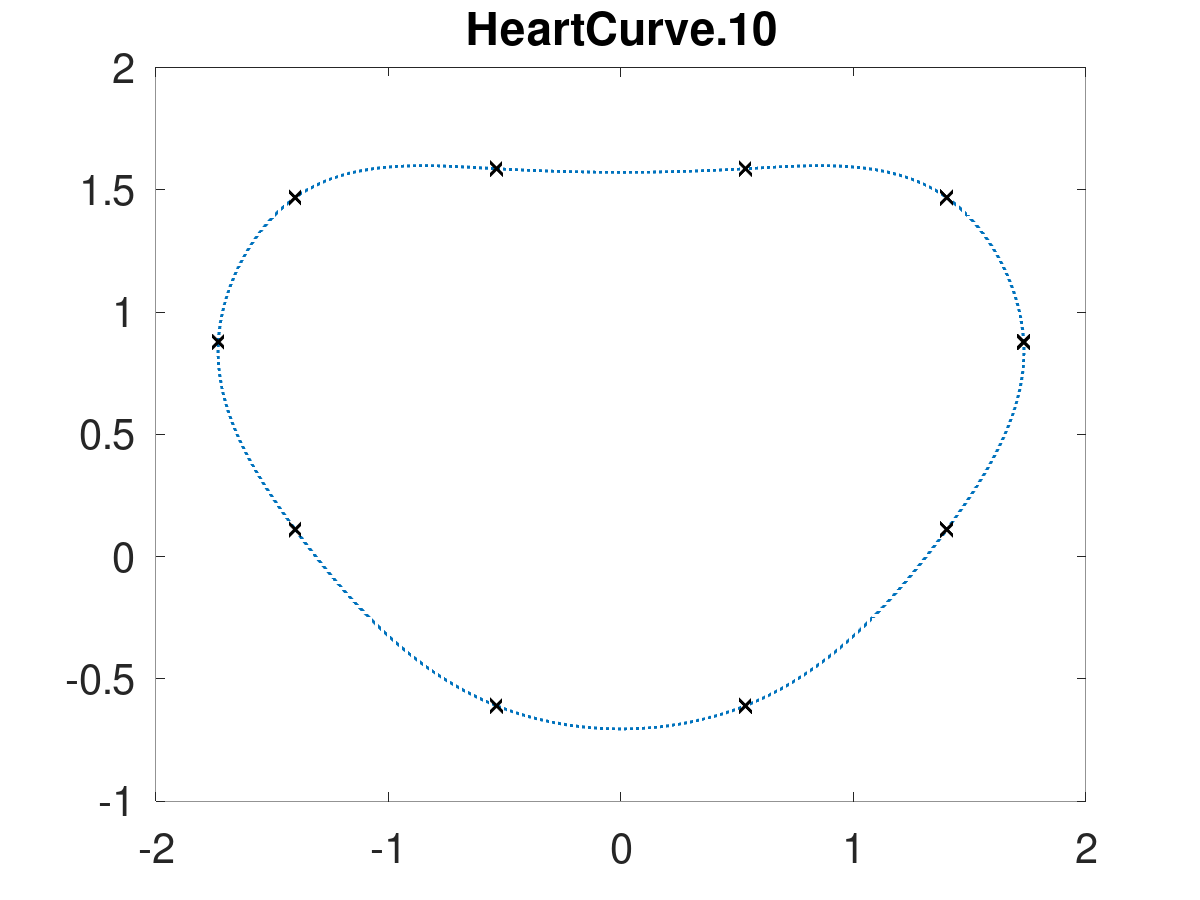
\includegraphics[width=0.45\textwidth]{../output/Assignment_E_10.png}
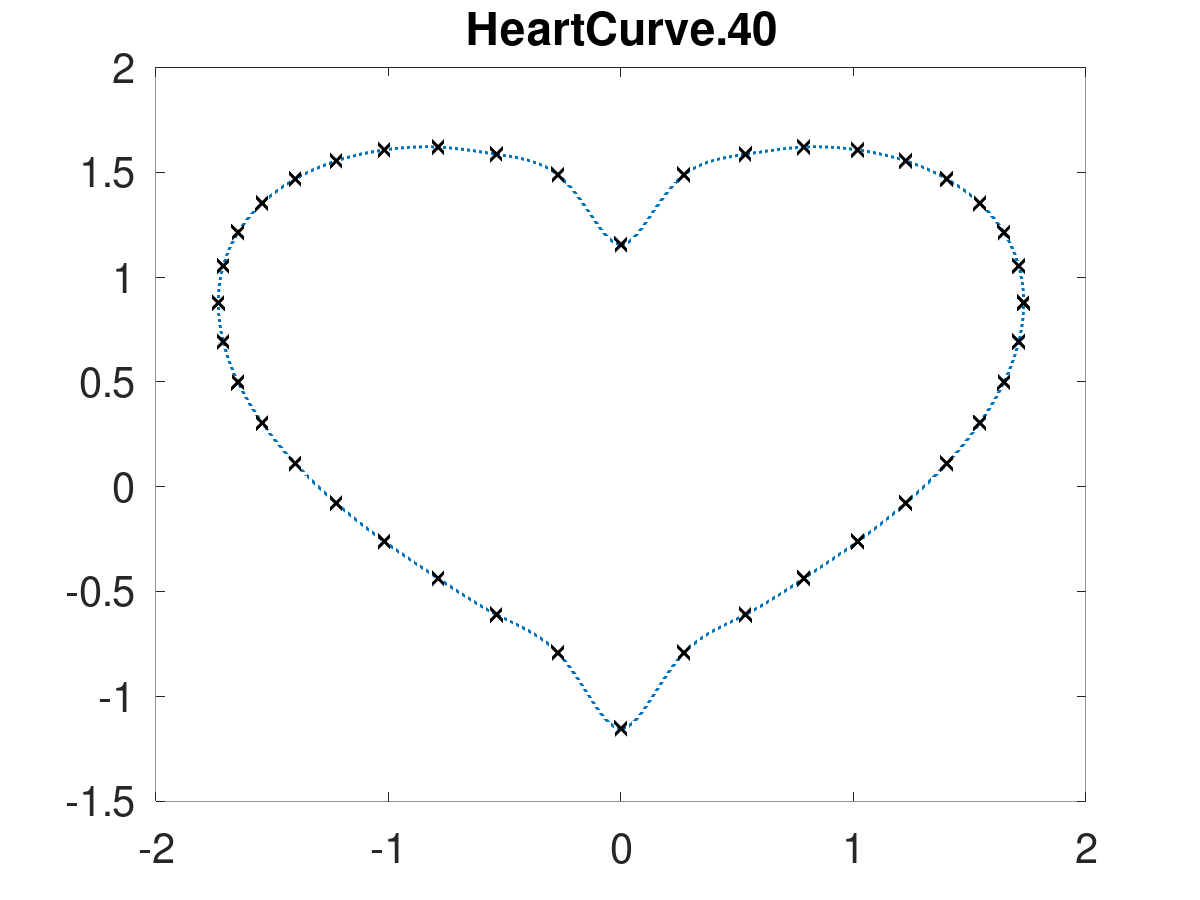
\includegraphics[width=0.45\textwidth]{../output/Assignment_E_40.png}

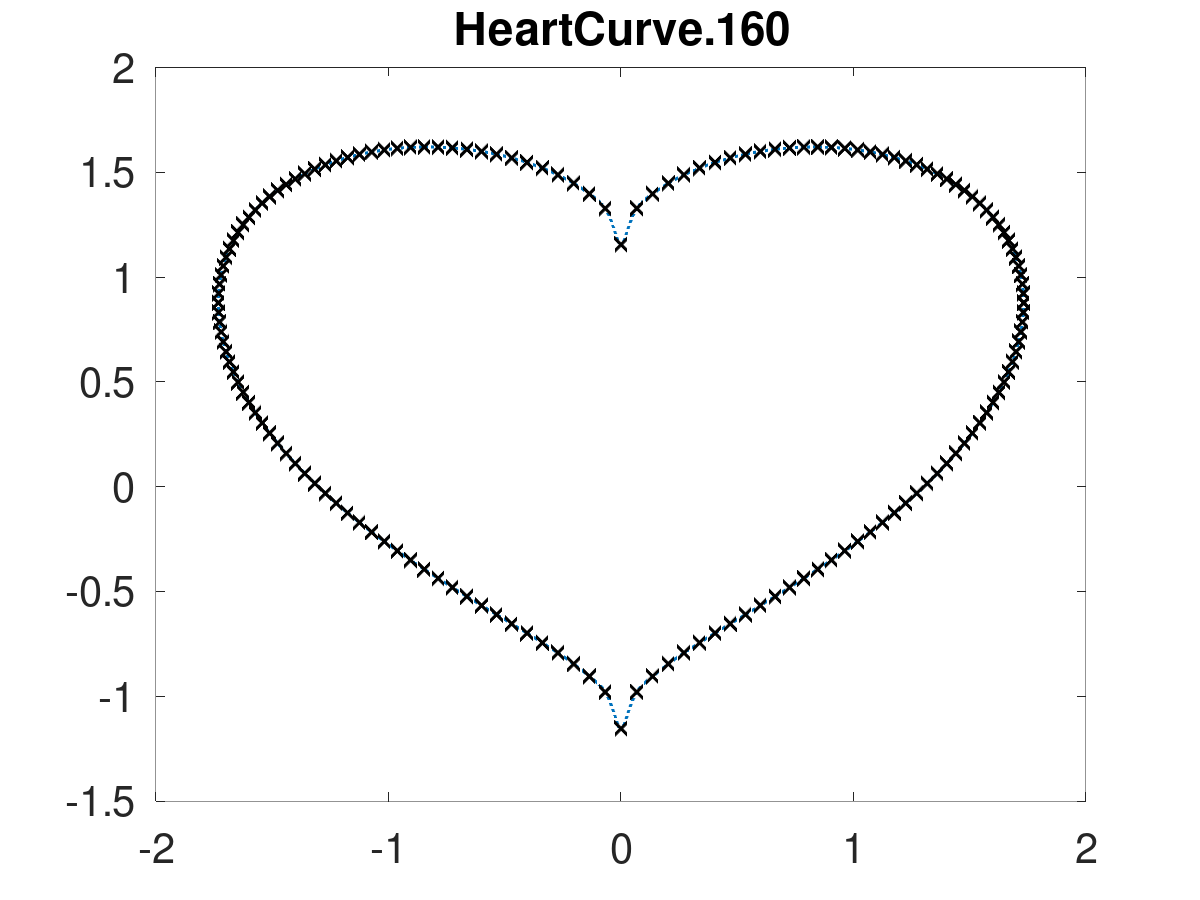
\includegraphics[width=0.5\textwidth]{../output/Assignment_E_160.png}

\subsection{\textbf{Assignment F}}
\lstset{language=C++}
\begin{lstlisting}
  ------------------------Assignment F--------------------------
  Plots have been generated as '/output/F_beastPlot.m'.
\end{lstlisting}
After plotting, we have

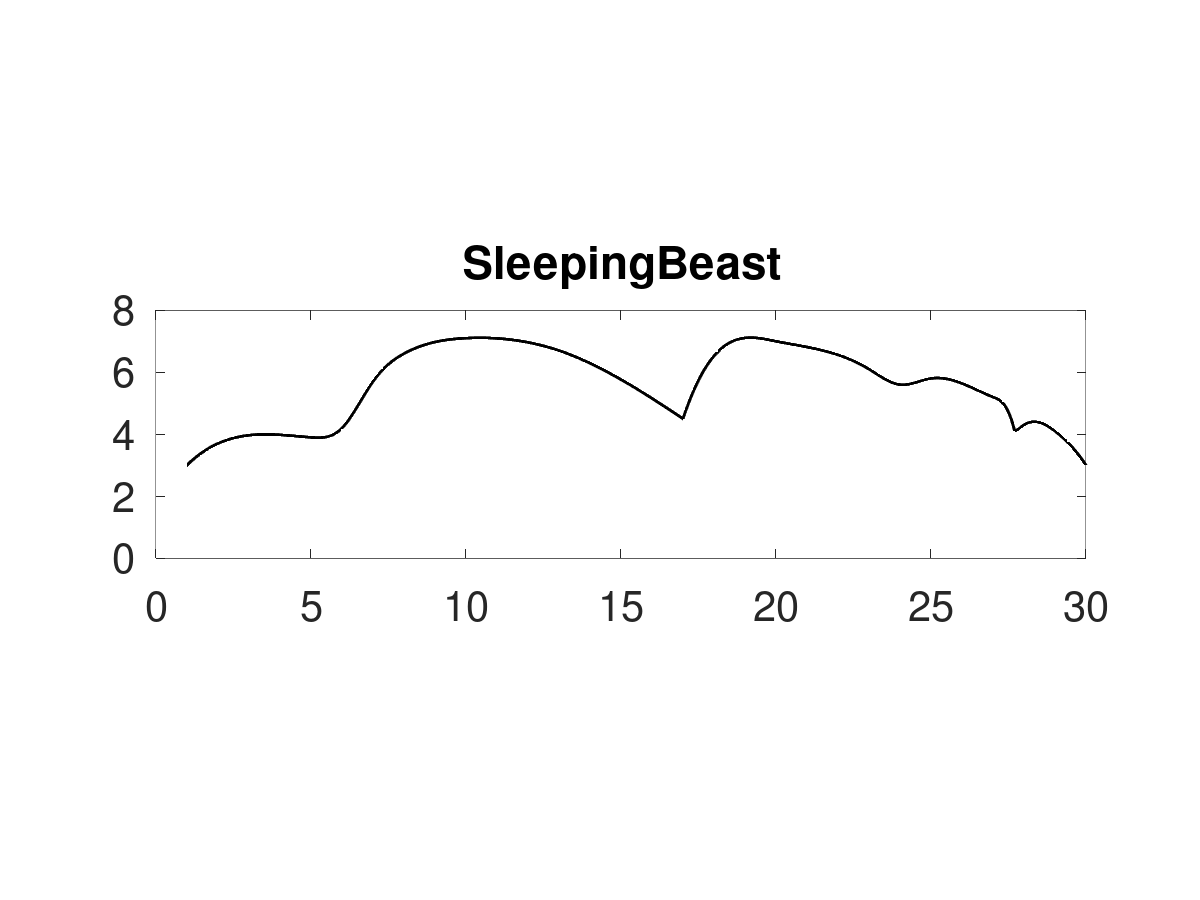
\includegraphics[width=0.5\textwidth]{../output/Assignment_F_beastPlot.png}


\subsection{\textbf{Assignment G}}
\lstset{language=C++}
\begin{lstlisting}
  ------------------------Assignment G--------------------------
  Plots have been generated as '/output/G_N[X].m'.
  
  ------------------------All Assignments Completed------------------------
\end{lstlisting}
After plotting, we have

\begin{figure}[!htbp]
  \flushleft
  \subfigure
  {
  \begin{minipage}[b]{.3\linewidth}
    \flushleft
  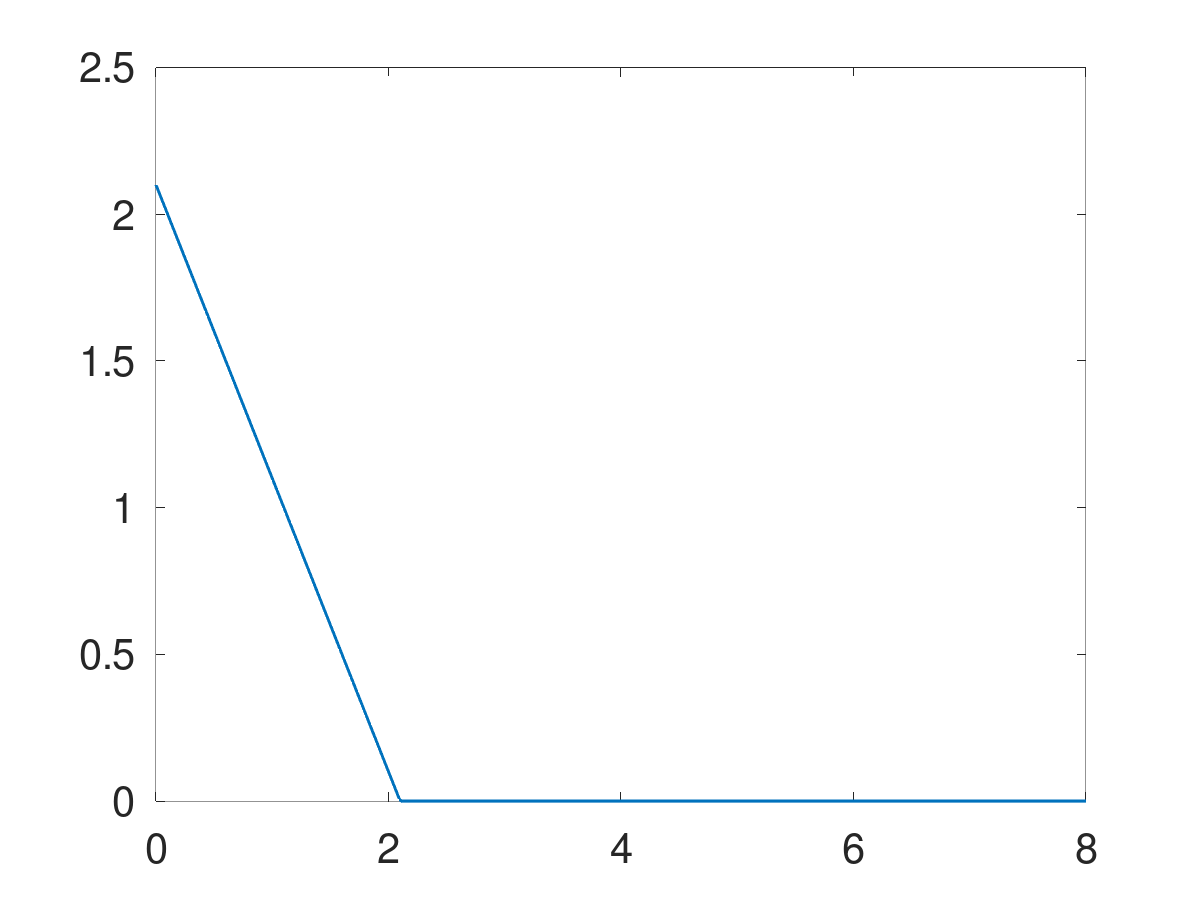
\includegraphics[scale=0.1]{../output/Assignment_G_N1_0_0.png}
  \end{minipage}
  }
  \subfigure
  {
  \begin{minipage}[b]{.3\linewidth}
    \flushleft
  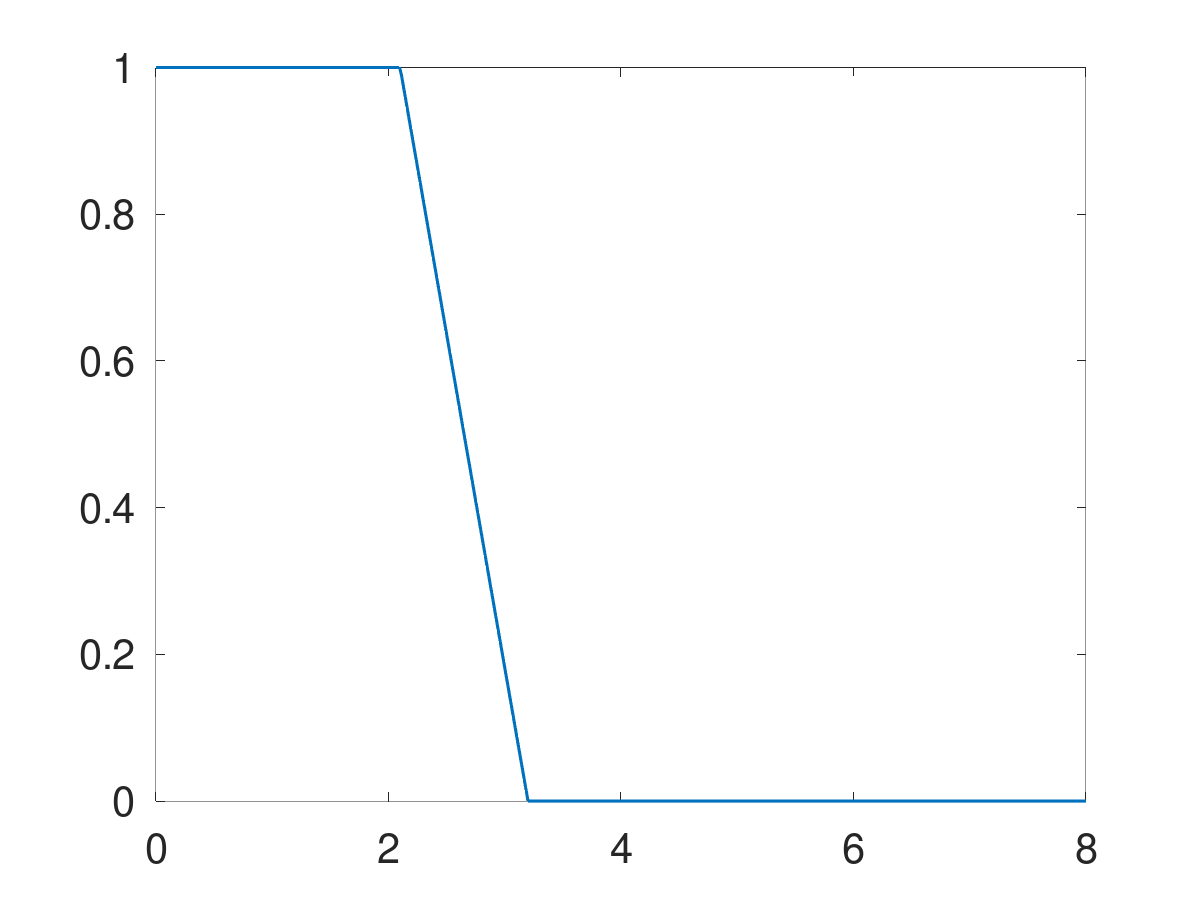
\includegraphics[scale=0.1]{../output/Assignment_G_N1_1_0.png}
  \end{minipage}
  }
  \subfigure
  {
  \begin{minipage}[b]{.3\linewidth}
    \flushleft
  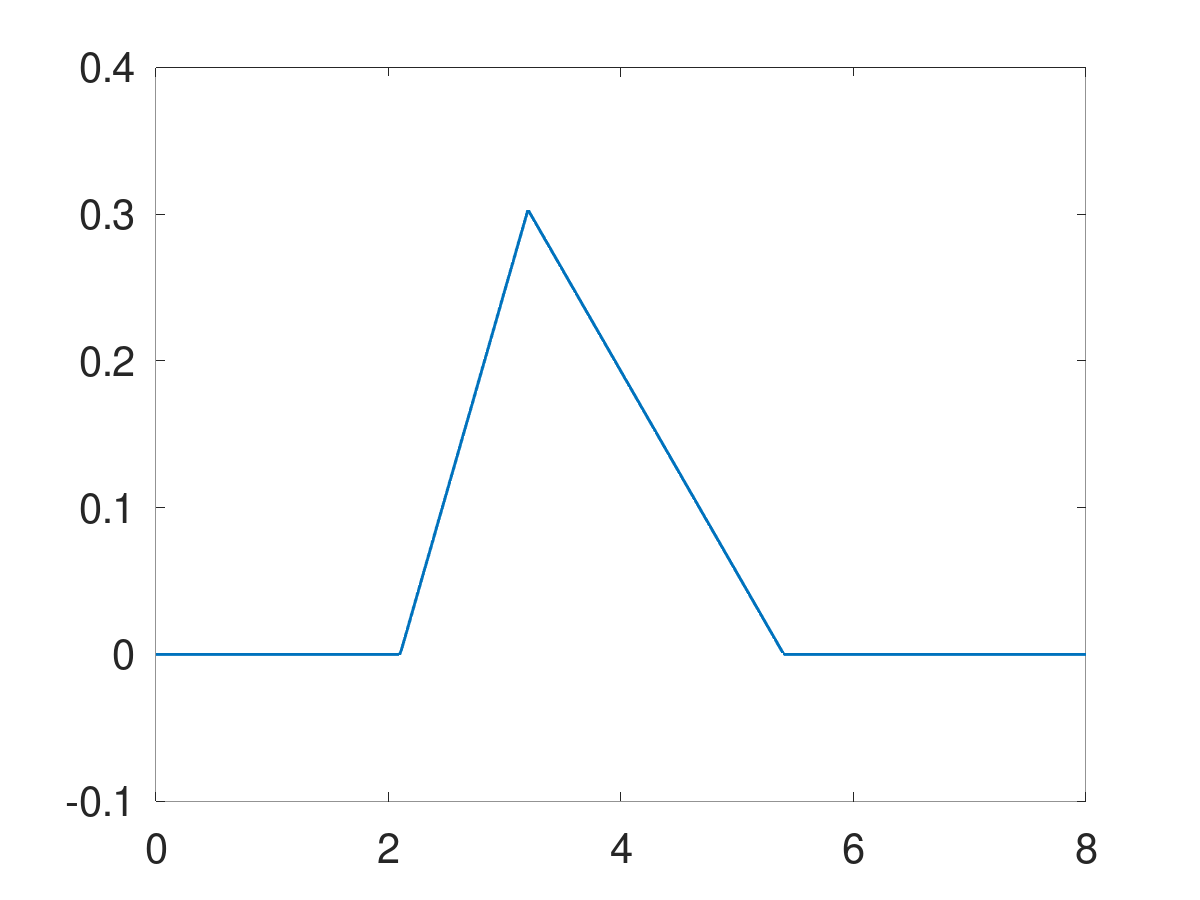
\includegraphics[scale=0.1]{../output/Assignment_G_N1_2_0.png}
  \end{minipage}
  }
  \subfigure
  {
  \begin{minipage}[b]{.3\linewidth}
    \flushleft
  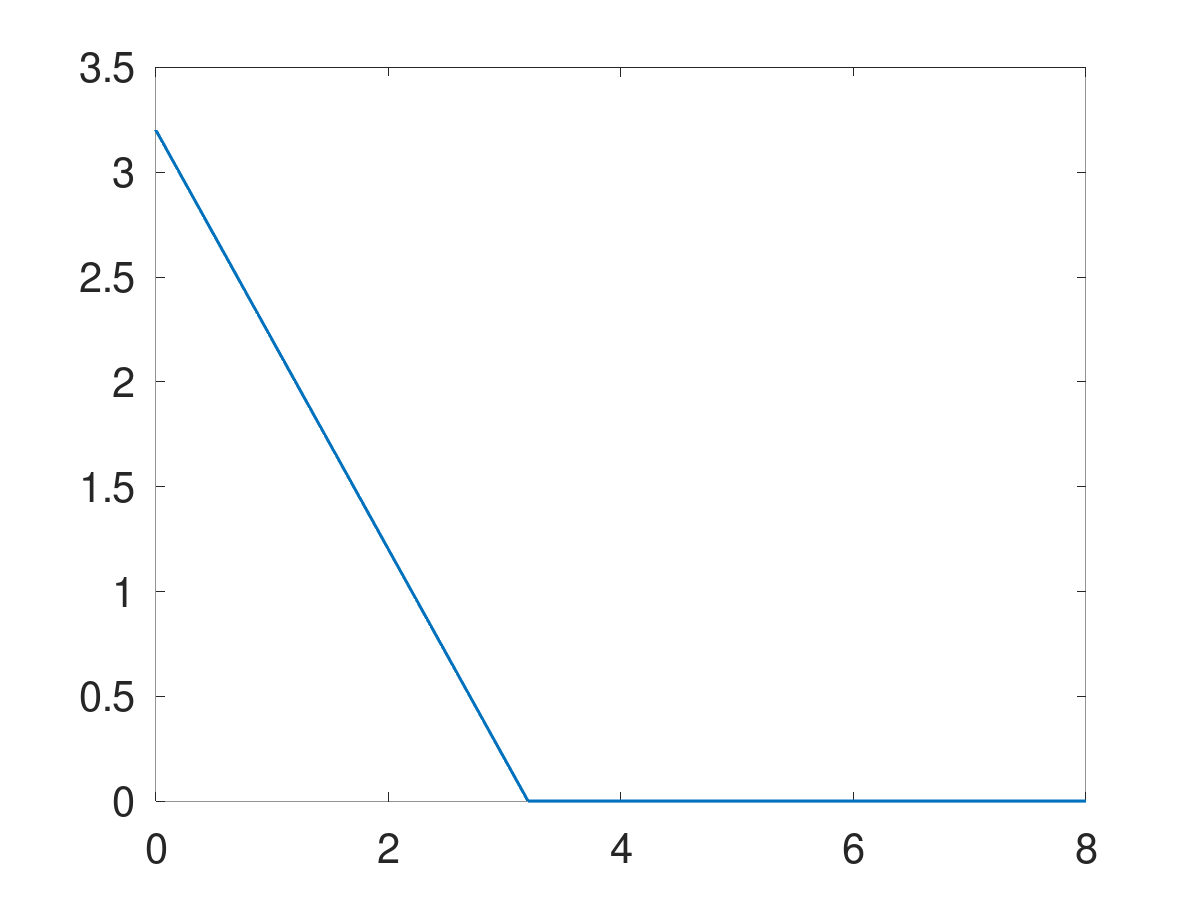
\includegraphics[scale=0.1]{../output/Assignment_G_N1_0_1.png}
  \end{minipage}
  }
  \subfigure{
  \begin{minipage}[b]{.3\linewidth}
    \flushleft
  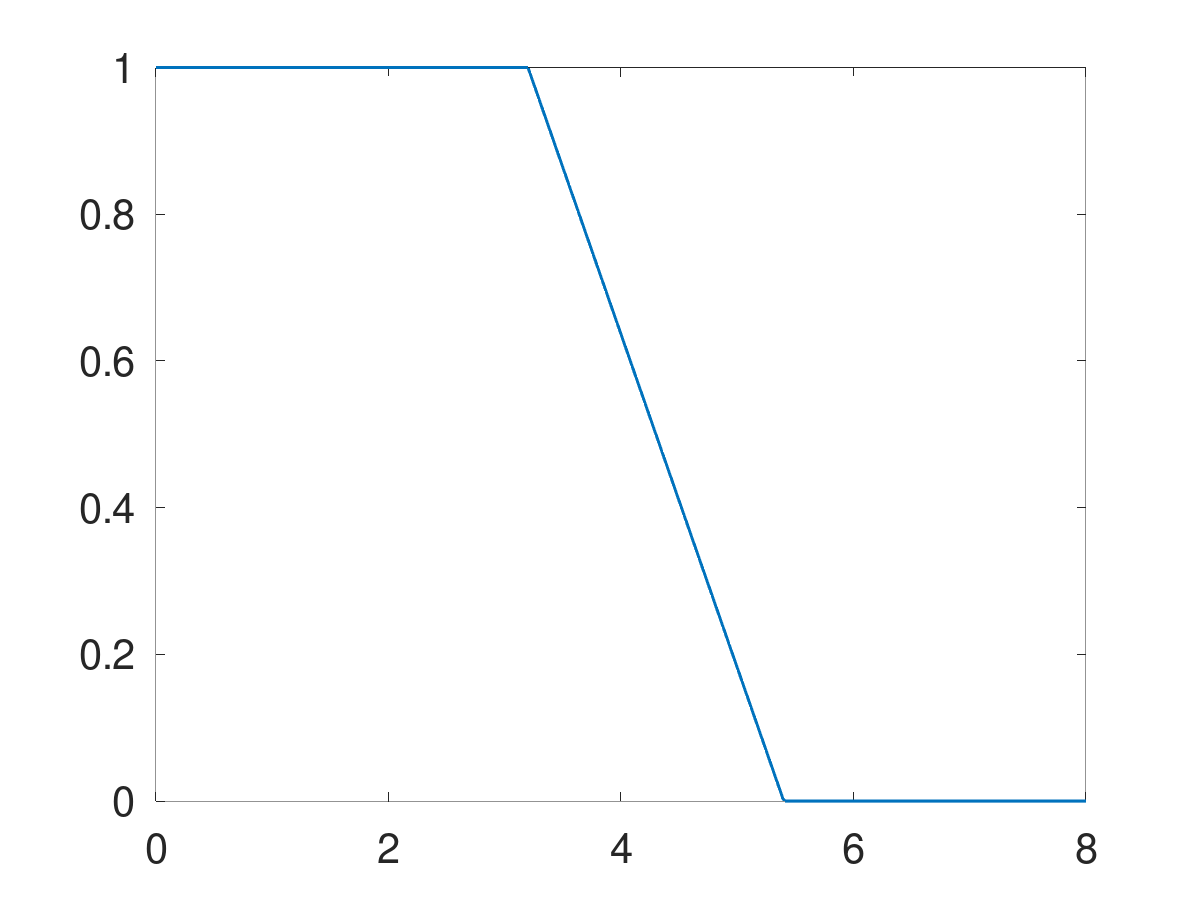
\includegraphics[scale=0.1]{../output/Assignment_G_N1_1_1.png}
  \end{minipage}
  }
  \newline
  \subfigure{
  \begin{minipage}[b]{.3\linewidth}
    \flushleft
  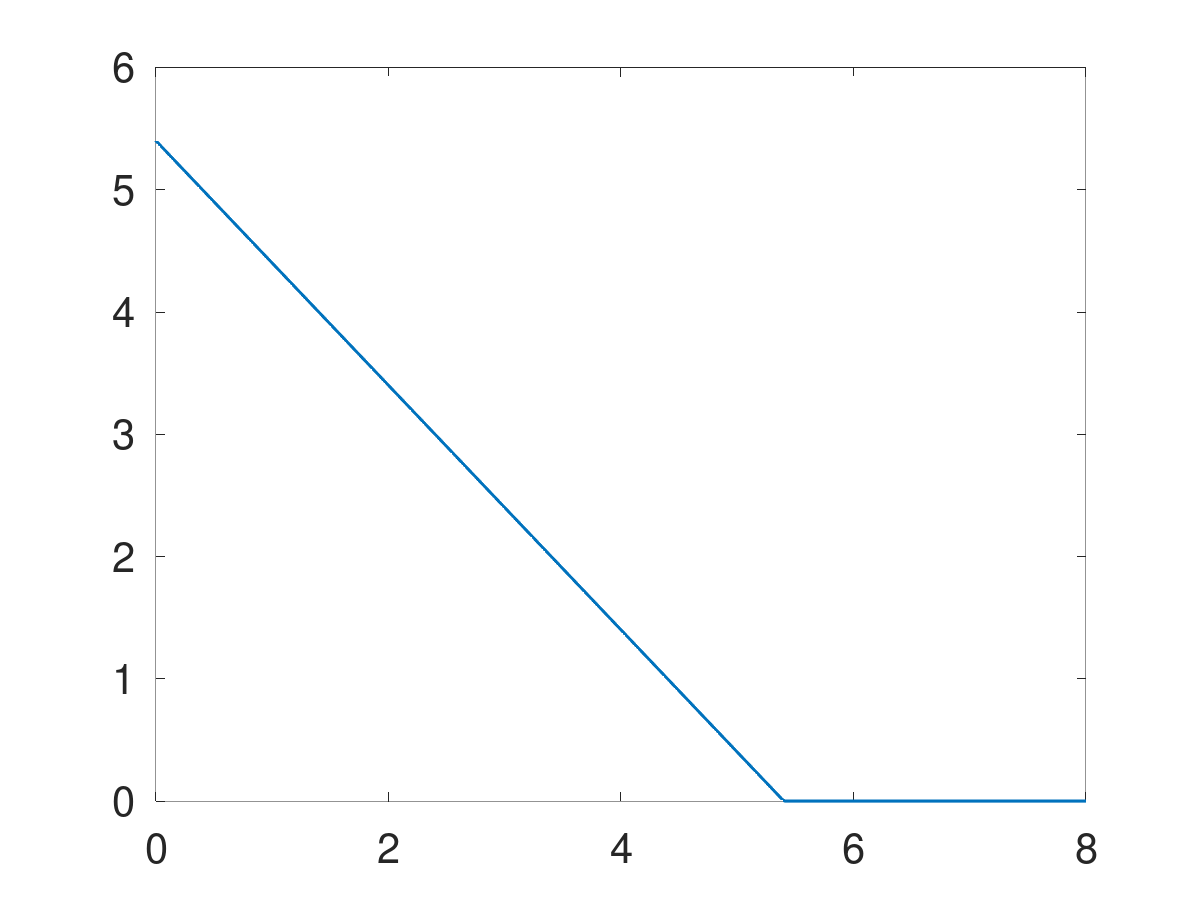
\includegraphics[scale=0.1]{../output/Assignment_G_N1_0_2.png}
  \end{minipage}
  }
  \caption{N=1}
  \end{figure}


  \begin{figure}[!htbp]
    \flushleft
    \subfigure
    {
    \begin{minipage}[b]{.23\linewidth}
      \flushleft
    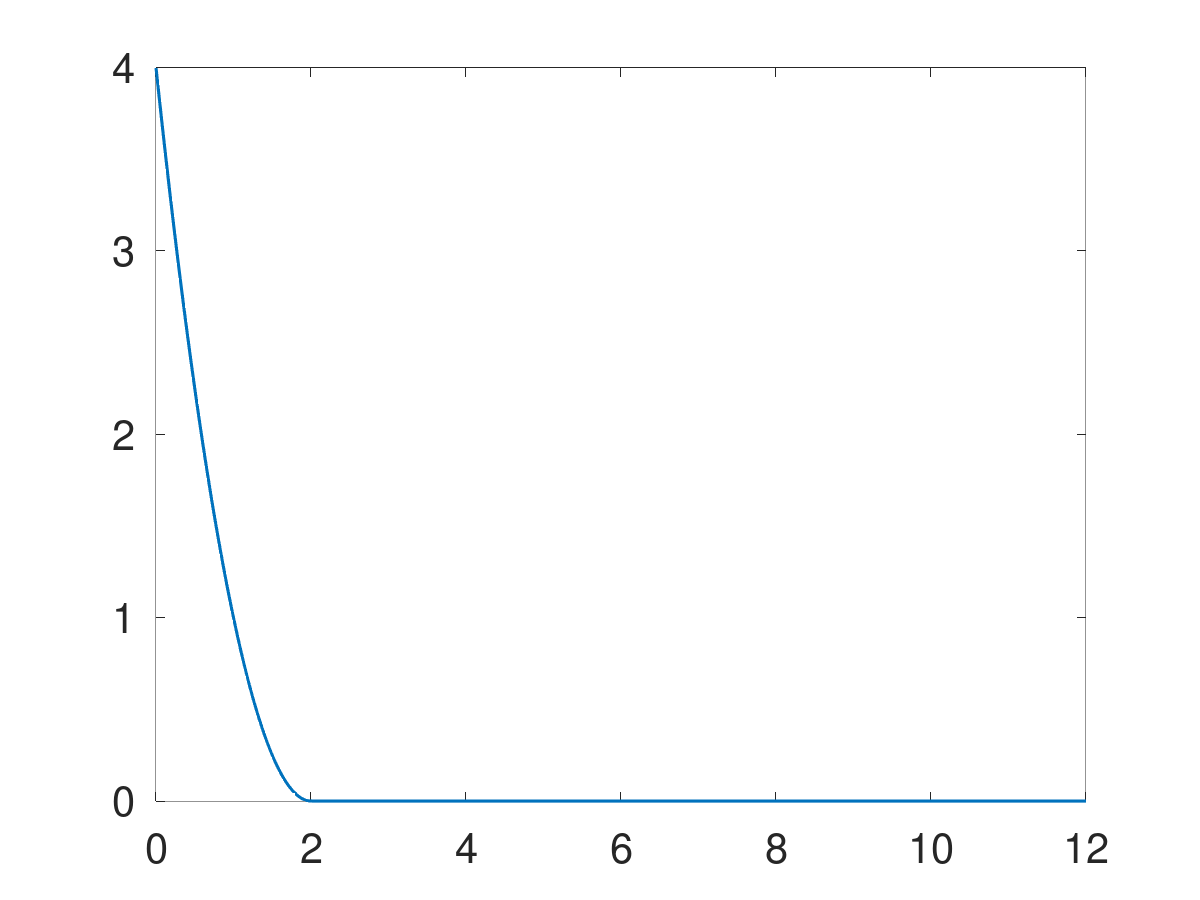
\includegraphics[scale=0.1]{../output/Assignment_G_N2_0_0.png}
    \end{minipage}
    }
    \subfigure
    {
    \begin{minipage}[b]{.23\linewidth}
      \flushleft
    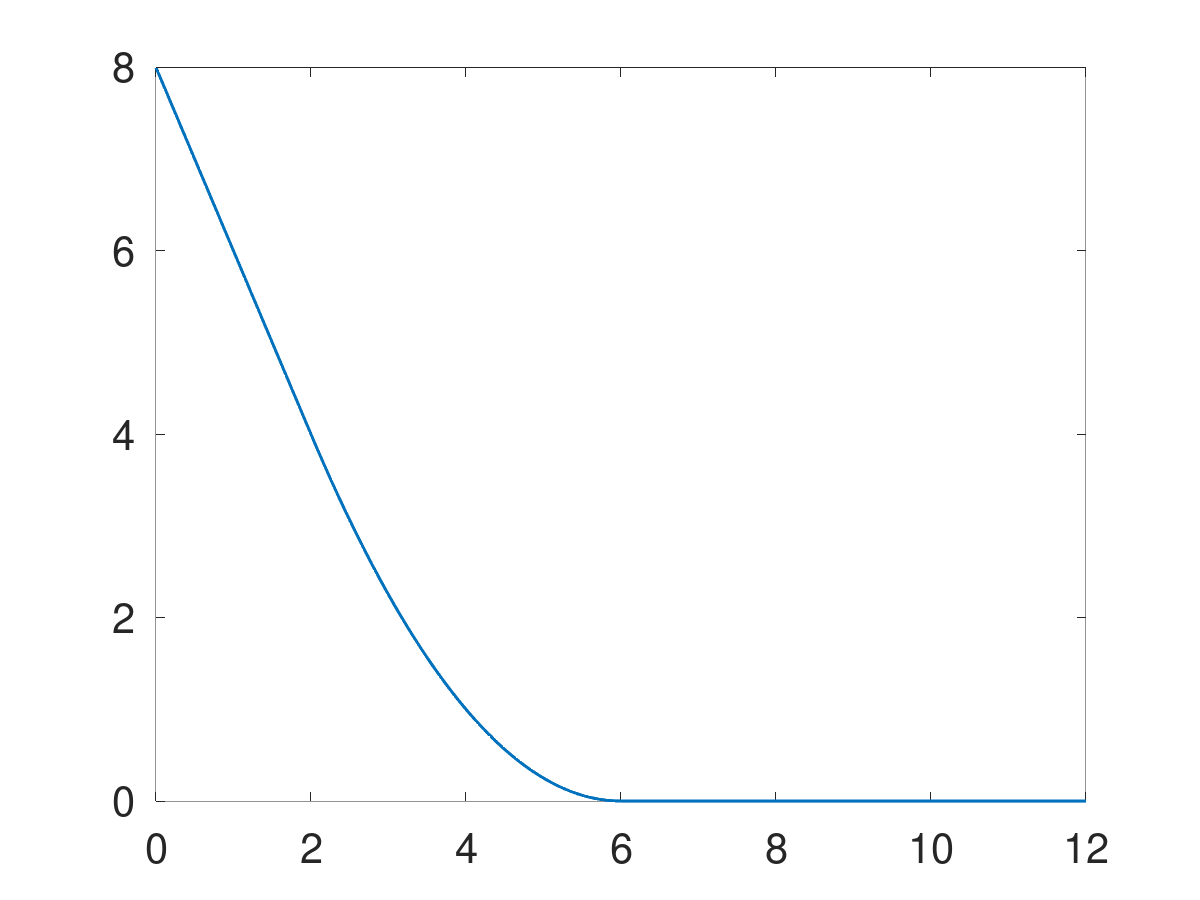
\includegraphics[scale=0.1]{../output/Assignment_G_N2_1_0.png}
    \end{minipage}
    }
    \subfigure
    {
    \begin{minipage}[b]{.23\linewidth}
      \flushleft
    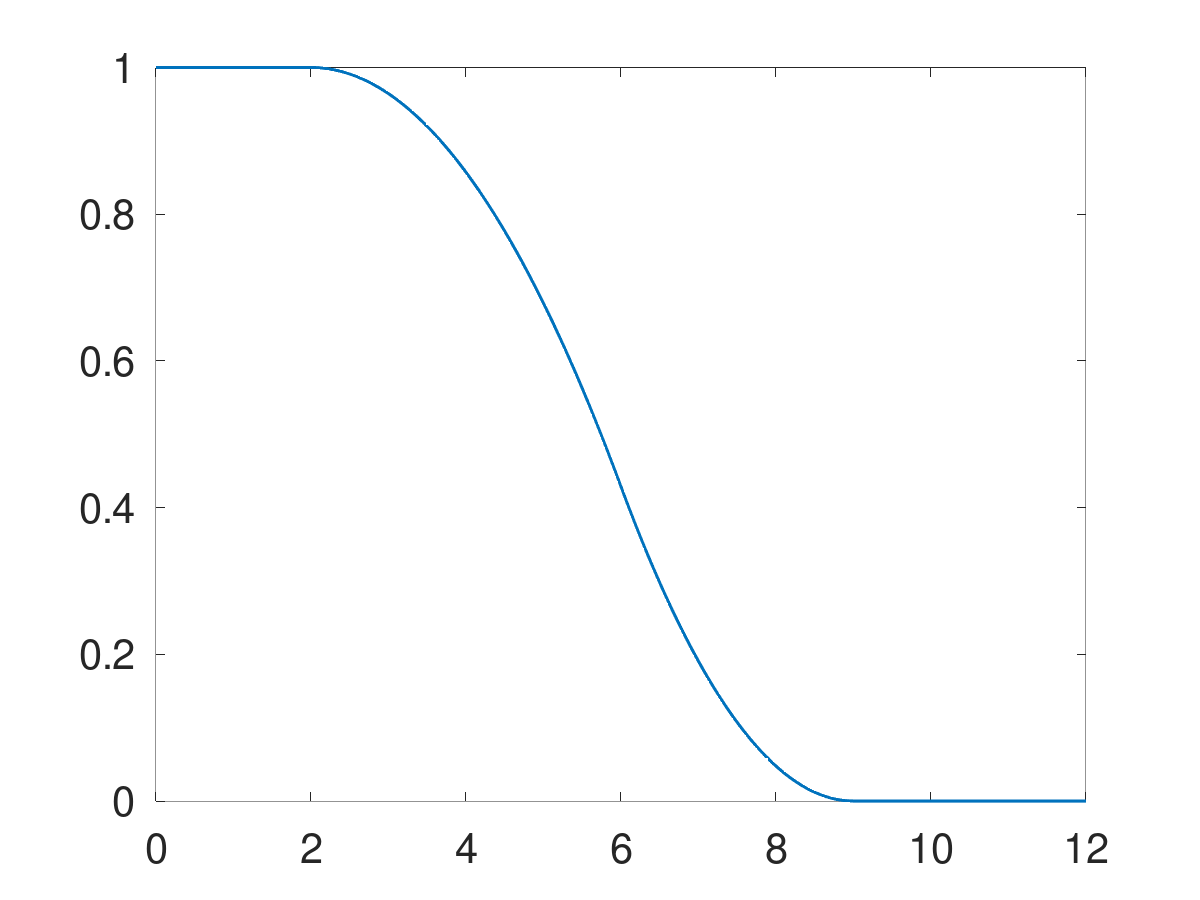
\includegraphics[scale=0.1]{../output/Assignment_G_N2_2_0.png}
    \end{minipage}
    }
    \subfigure
    {
    \begin{minipage}[b]{.23\linewidth}
      \flushleft
    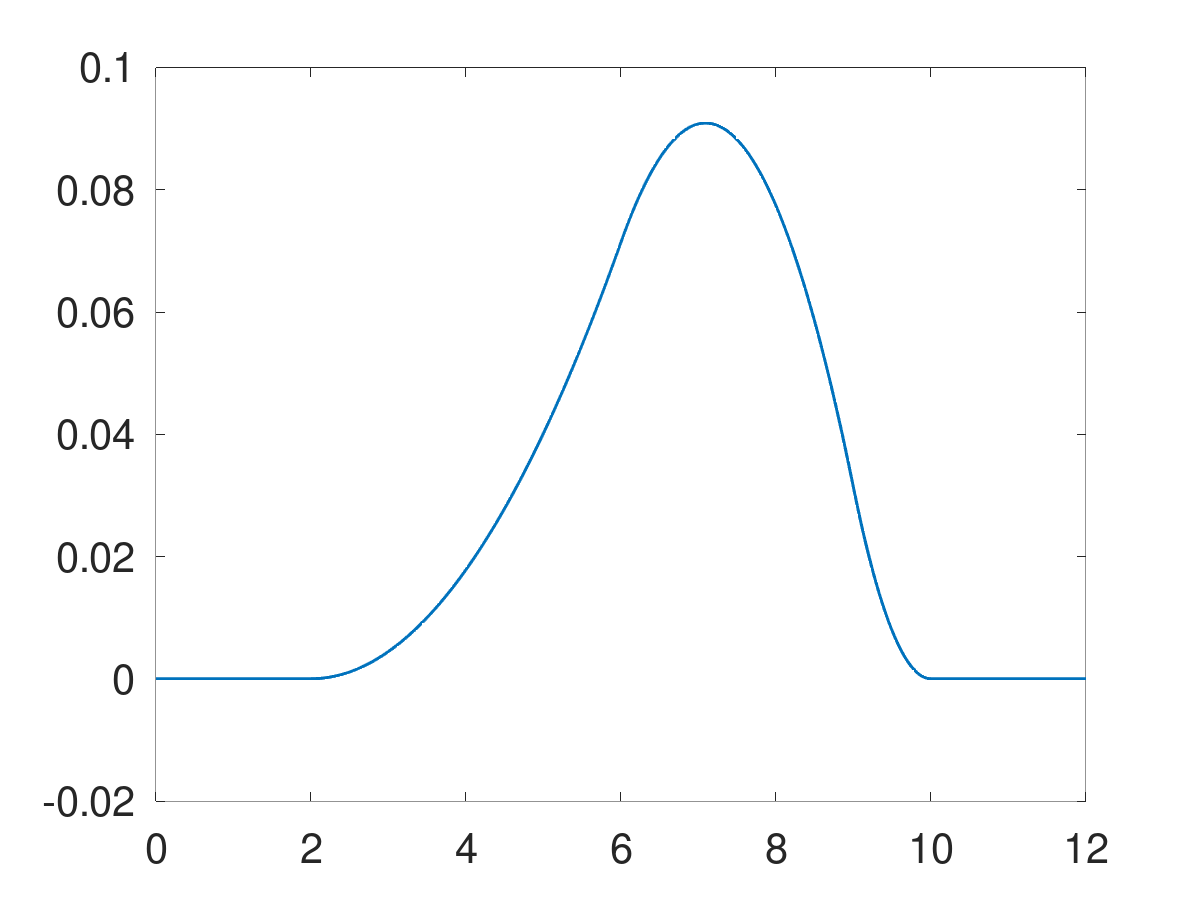
\includegraphics[scale=0.1]{../output/Assignment_G_N2_3_0.png}
    \end{minipage}
    }
    \newline
    \subfigure{
    \begin{minipage}[b]{.23\linewidth}
      \flushleft
    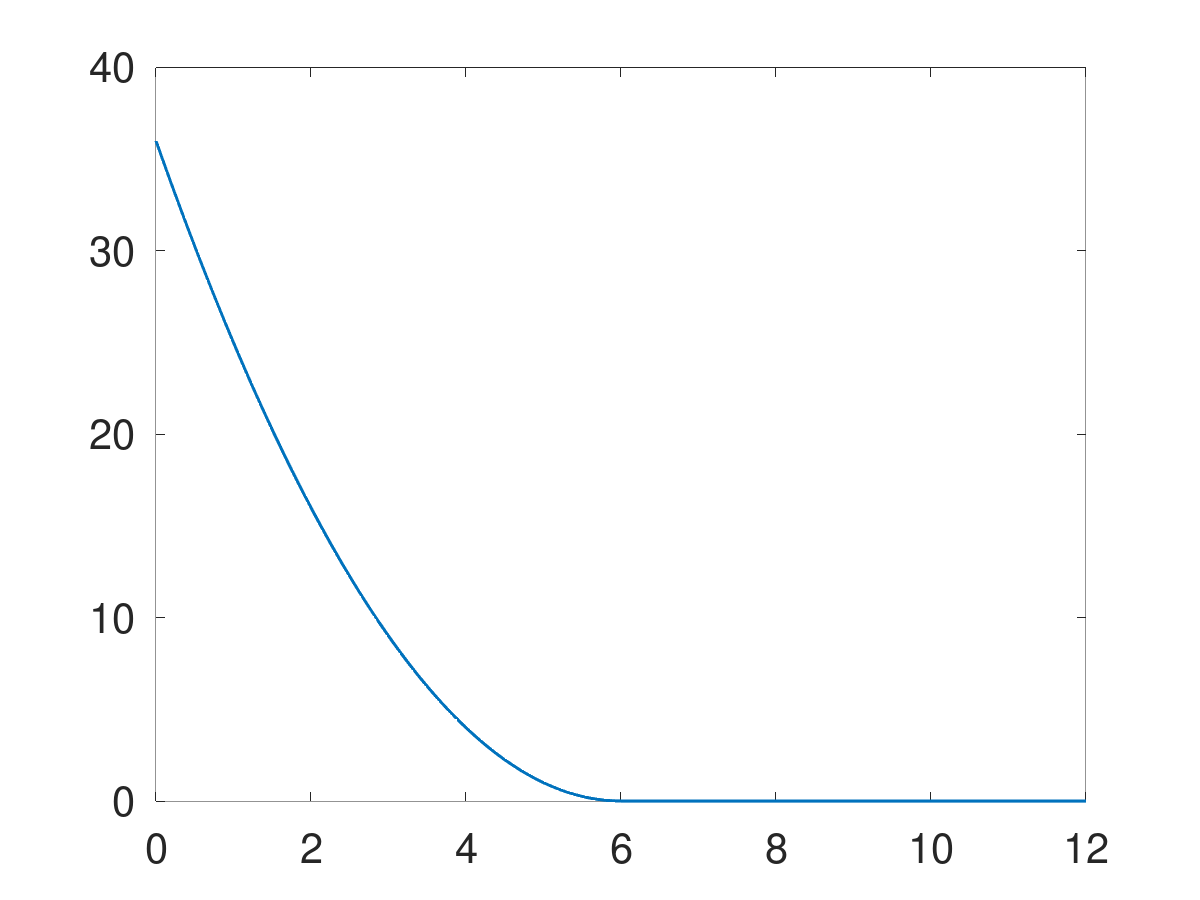
\includegraphics[scale=0.1]{../output/Assignment_G_N2_0_1.png}
    \end{minipage}
    }
    \subfigure{
    \begin{minipage}[b]{.23\linewidth}
      \flushleft
    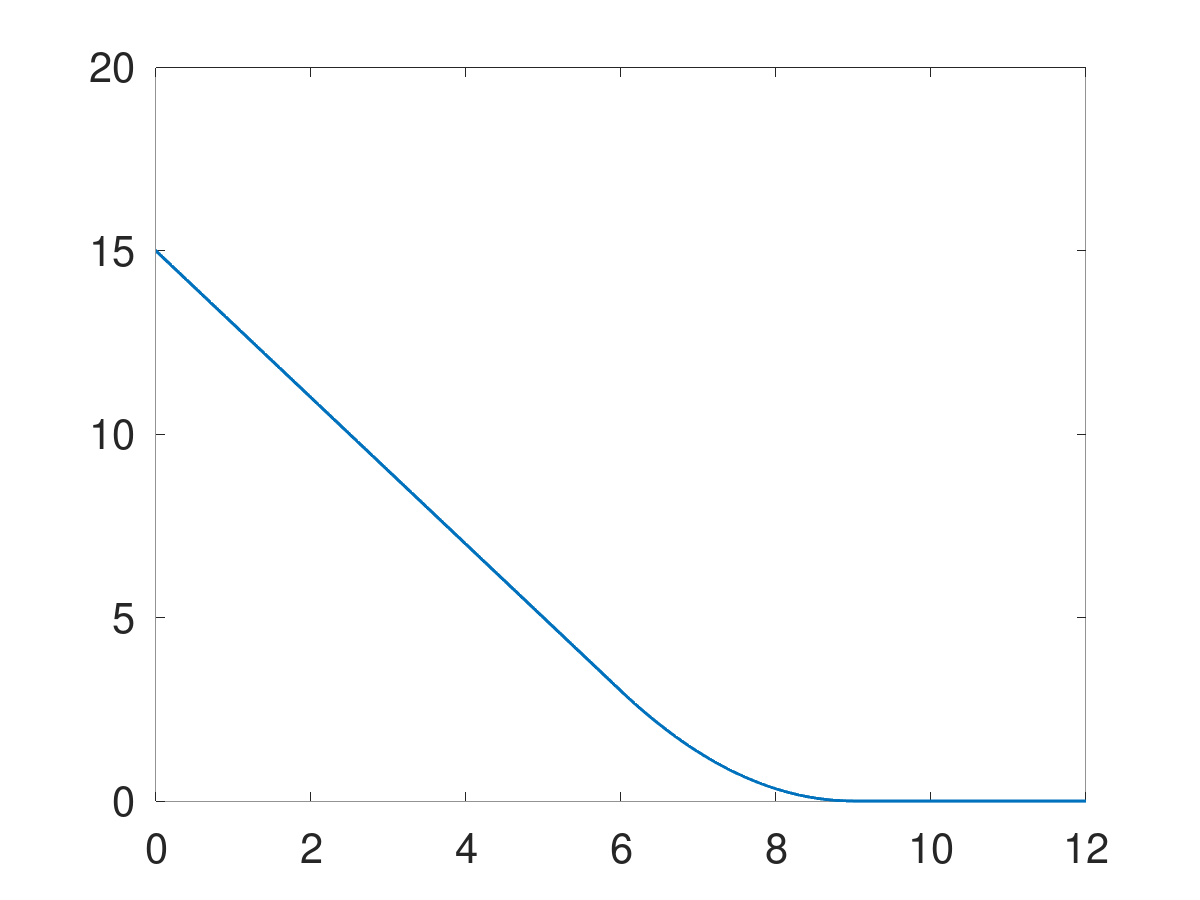
\includegraphics[scale=0.1]{../output/Assignment_G_N2_1_1.png}
    \end{minipage}
    }
    \subfigure{
      \begin{minipage}[b]{.23\linewidth}
        \flushleft
      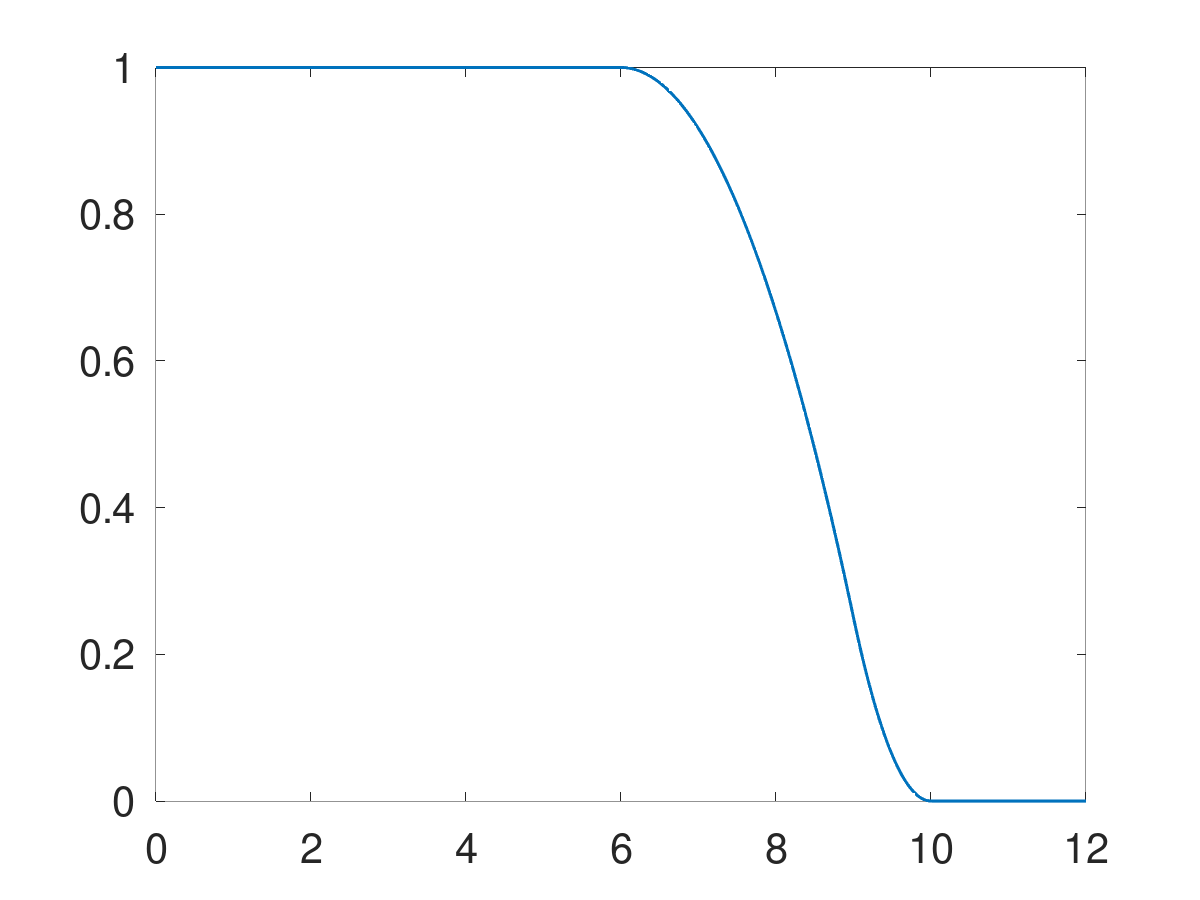
\includegraphics[scale=0.1]{../output/Assignment_G_N2_2_1.png}
      \end{minipage}
    }
    \newline
    \subfigure{
      \begin{minipage}[b]{.23\linewidth}
        \flushleft
      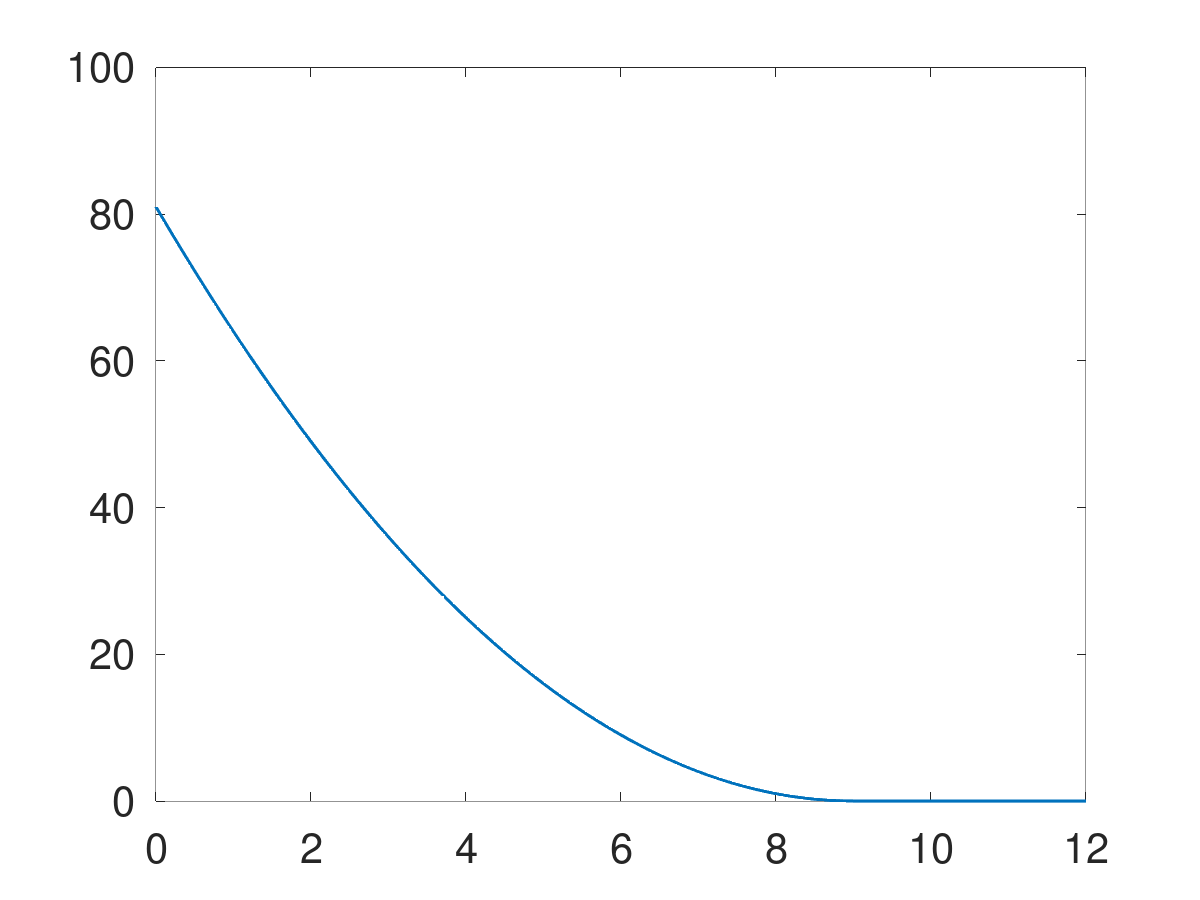
\includegraphics[scale=0.1]{../output/Assignment_G_N2_0_2.png}
      \end{minipage}
    }
    \subfigure{
    \begin{minipage}[b]{.23\linewidth}
      \flushleft
    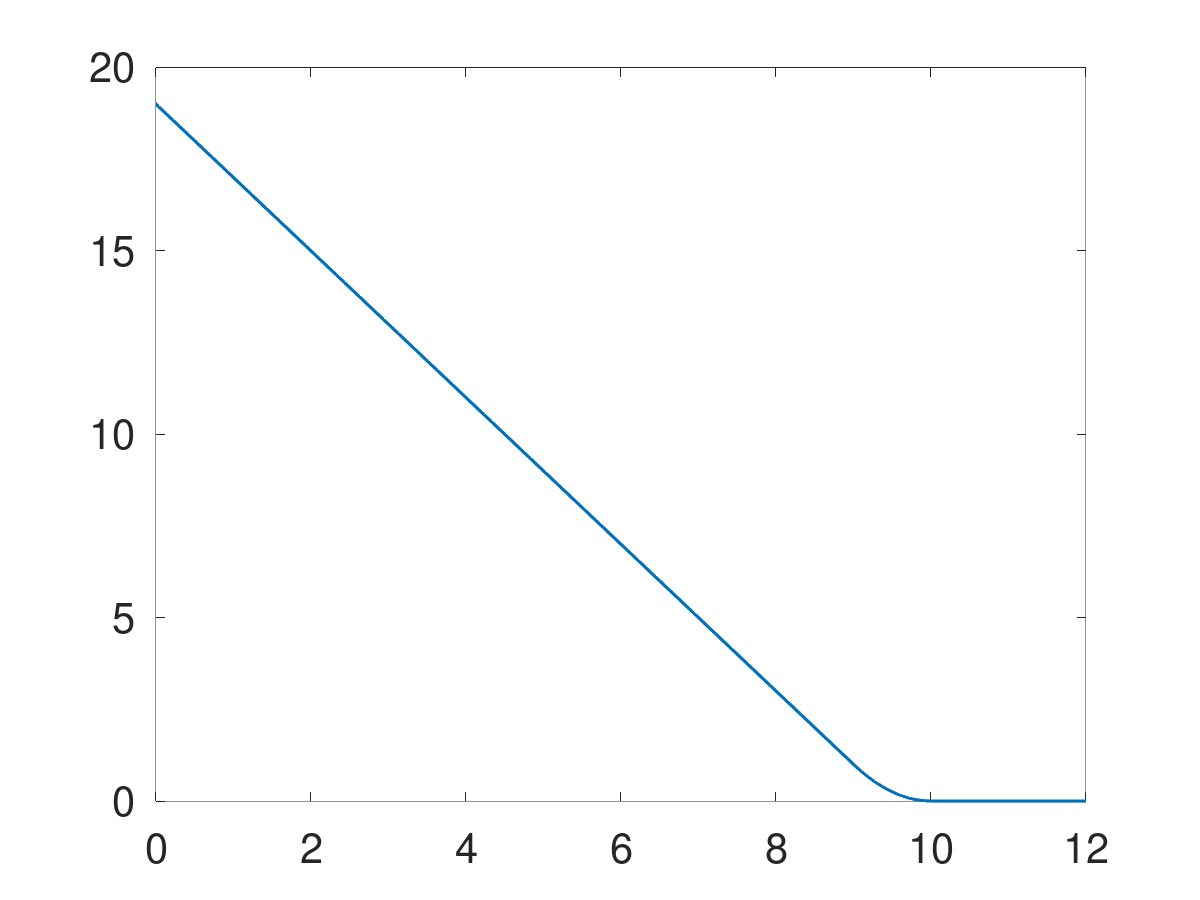
\includegraphics[scale=0.1]{../output/Assignment_G_N2_1_2.png}
    \end{minipage}
    }
    \newline
    \subfigure{
    \begin{minipage}[b]{.23\linewidth}
      \flushleft
    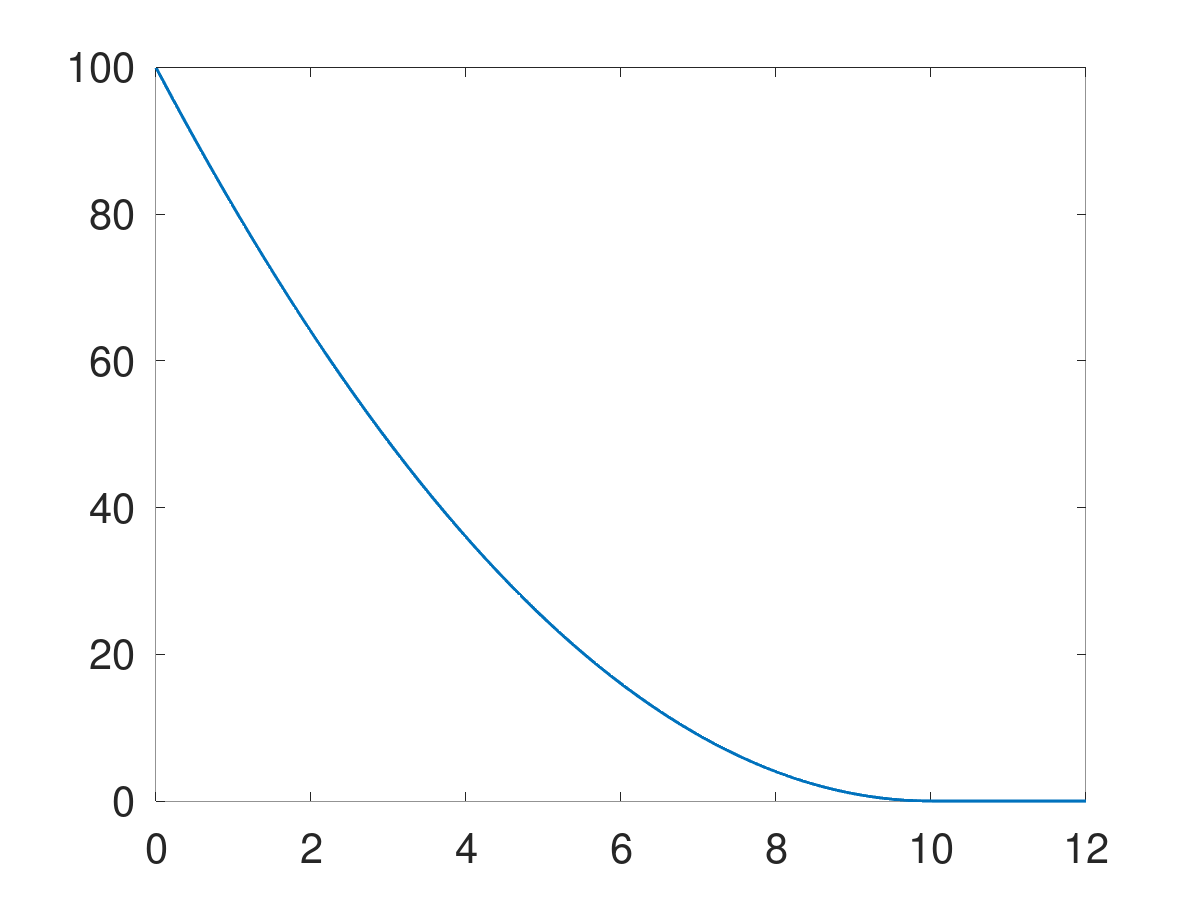
\includegraphics[scale=0.1]{../output/Assignment_G_N2_0_3.png}
    \end{minipage}
    } 
    \caption{N=2}
    \end{figure}
\newpage

    Then comparing them with B-splines that are retracted by factor $t_{i+n}-t_{i-1}$ 
    yields

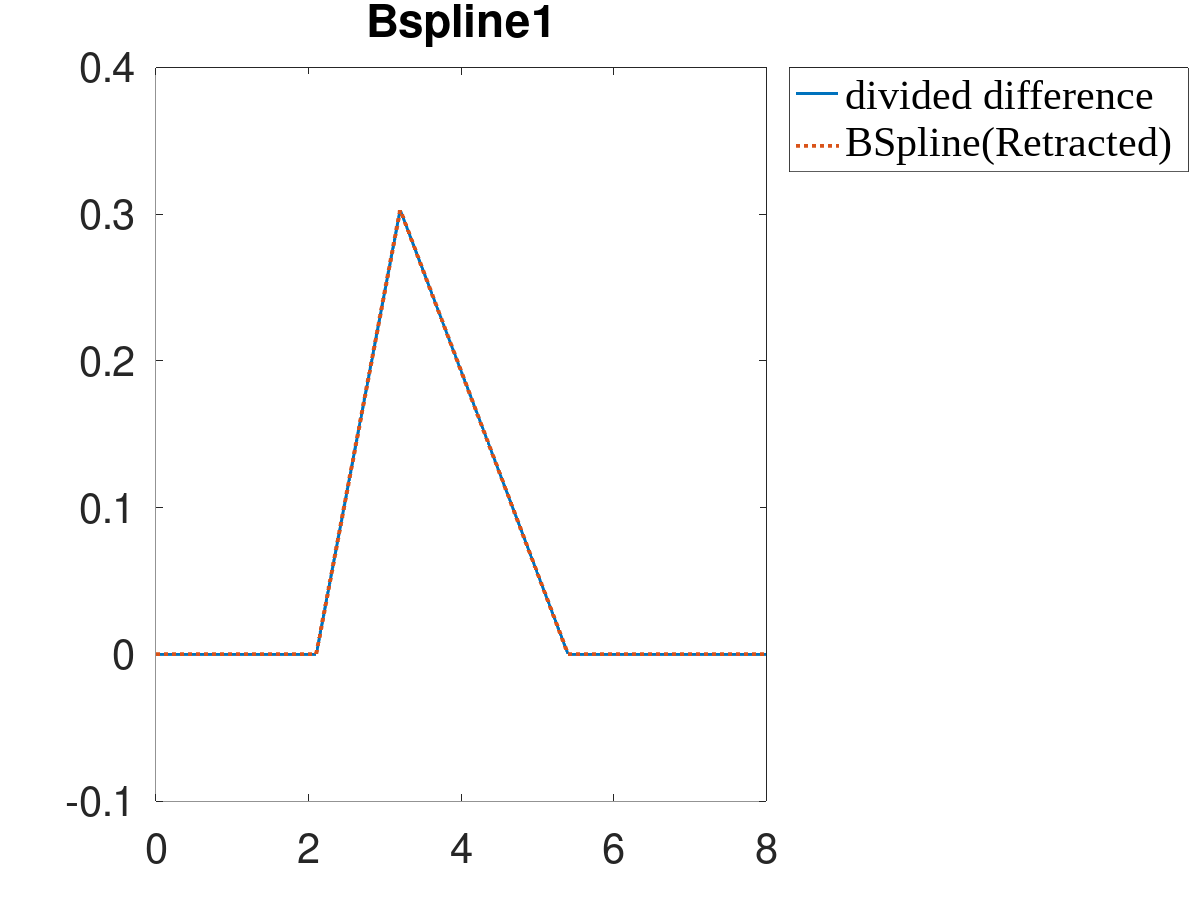
\includegraphics[width=0.45\textwidth]{../output/Assignment_G_1_Compare.png}
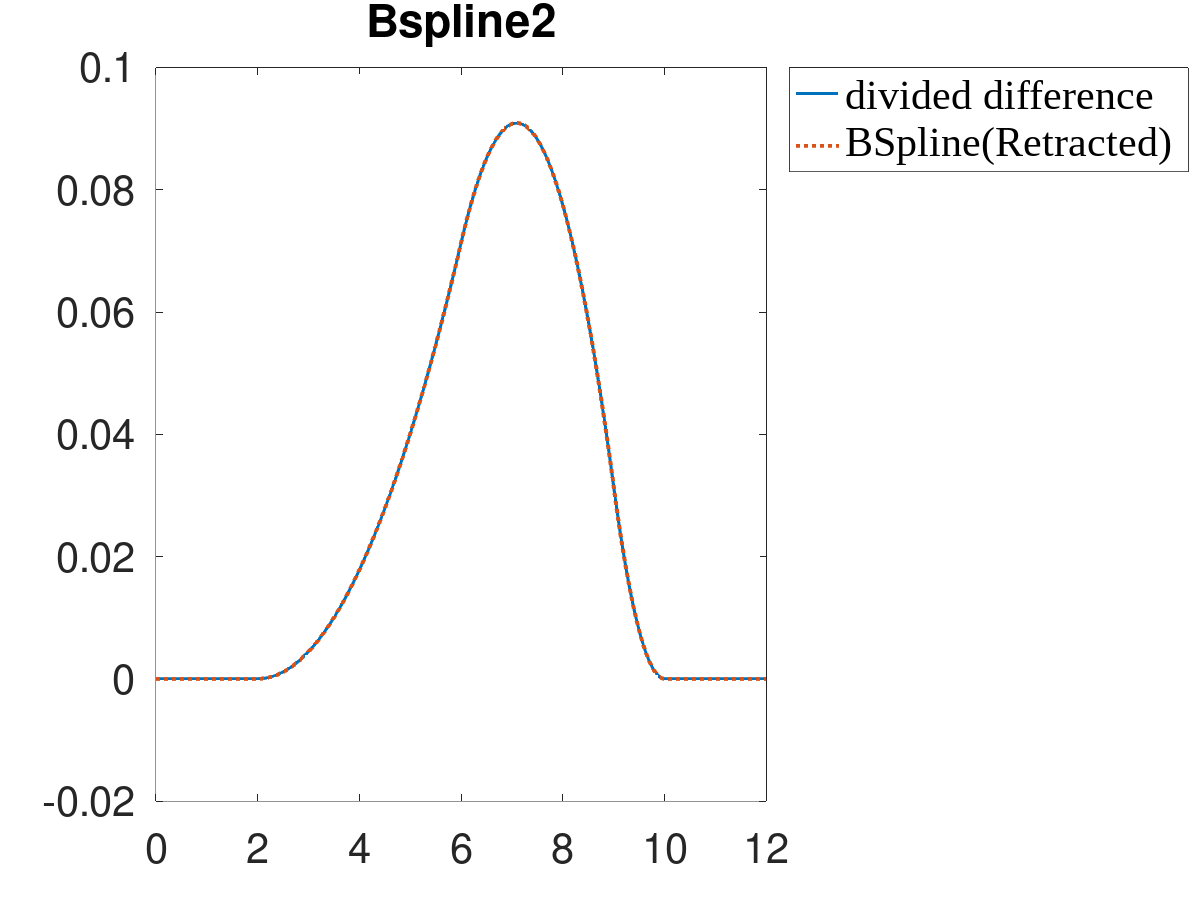
\includegraphics[width=0.45\textwidth]{../output/Assignment_G_2_Compare.png}

which corresponds to the theorem.

\end{document}
%%% Local Variables: 
%%% mode: latex
%%% TeX-master: t
%%% End: 
